
\documentclass[9pt]{beamer}

\usepackage[latin1]{inputenc}
\usepackage{colortbl}
\usepackage[english]{babel}

\pgfdeclareimage[height=1.5cm]{logo-golab2019}{logo-golab2019}
\logo{\pgfuseimage{logo-golab2019}}

\newcommand{\myblue} [1] {{\color{blue}#1}}
\newcommand{\newauthor}[4]{
  \parbox{0.26\textwidth}{
    \texorpdfstring
      {
        \centering
        #1 \\
        \myblue{{\href{#2}{\texttt{#3}}}} \\
        #4 \\
      }
      {#1}
  }
}


% for code colouring
\usepackage{minted}
\definecolor{bg}{rgb}{0.95,0.95,0.95}
\setminted{bgcolor=bg}


% beamer template
\beamertemplatetransparentcovereddynamic
\usetheme{GoLabIO}
\definecolor{GoLabIOYellow}{RGB}{249,195,62}
\usecolortheme[named=GoLabIOYellow]{structure}

\usepackage[T1]{fontenc}
\usepackage{montserrat}

\hypersetup{%
  pdftitle={Go-HEP: what can Go do for science?},%
   pdfauthor={S\'ebastien Binet},%
%
}

\title[Go-HEP: what can Go do for science?]{Go-HEP: what can Go do for science?}
\date{2019-10-22}
\author[S\'ebastien Binet]{
 \parbox{0.26\textwidth}{
	\texorpdfstring
	  {
		\centering
 		S\'ebastien Binet \\
 		CNRS/IN2P3 \\
 		\myblue{\href{http://twitter.com/0xbins}{\texttt{@0xbins}}} \\
 		\myblue{\href{mailto:binet@cern.ch}{\texttt{binet@cern.ch}}} \\
 	  }
	{S\'ebastien Binet}
}
 }
\institute[GoLab-2019]{\insertlogo\hskip0.1cm}



\begin{document}

\frame{\titlepage
}

\part<presentation>{Main Talk}

\section[slides]{slides}

\begin{frame}[fragile]
\frametitle{High Energy Physics (HEP)}


	\begin{exampleblock}{}
Field of physics which studies the fundamental laws of Nature and the
properties of the constituents of matter.
	\end{exampleblock}{}


Many labs working on HEP around the world. 
But, perhaps one of the most famous ones is \myblue{\href{http://cern.ch}{\texttt{CERN}}}.



\end{frame}

\begin{frame}[fragile]
\frametitle{CERN}


\begin{figure}[h]
\begin{center}
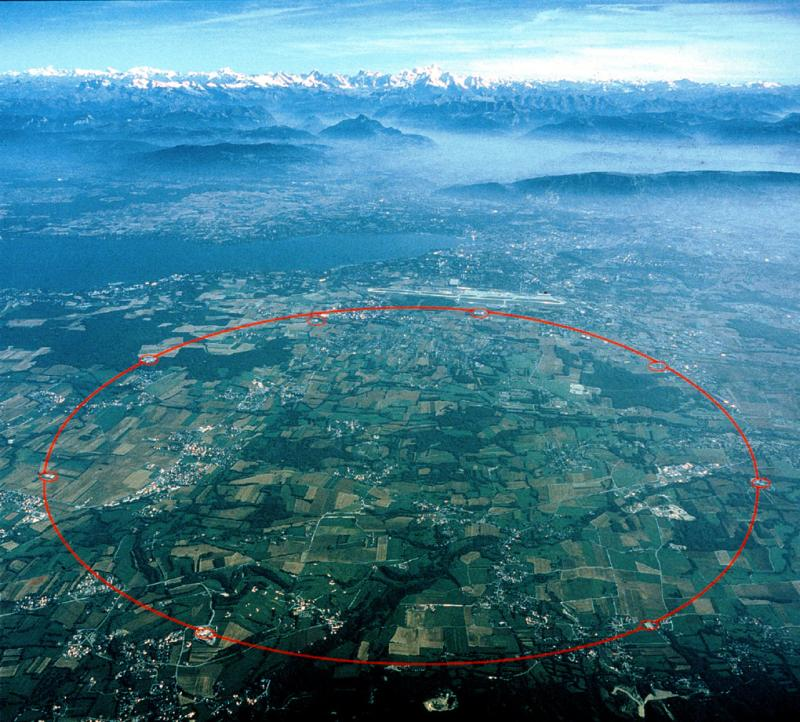
\includegraphics[width=9cm,height=6cm]{_figs/cernaerial.jpg}
\end{center}
	\caption{Aerial view of \texttt{CERN} \& \texttt{LHC}}

\end{figure}


\end{frame}

\begin{frame}[fragile]
\frametitle{CERN-LHC}

\begin{figure}[h]
\begin{center}
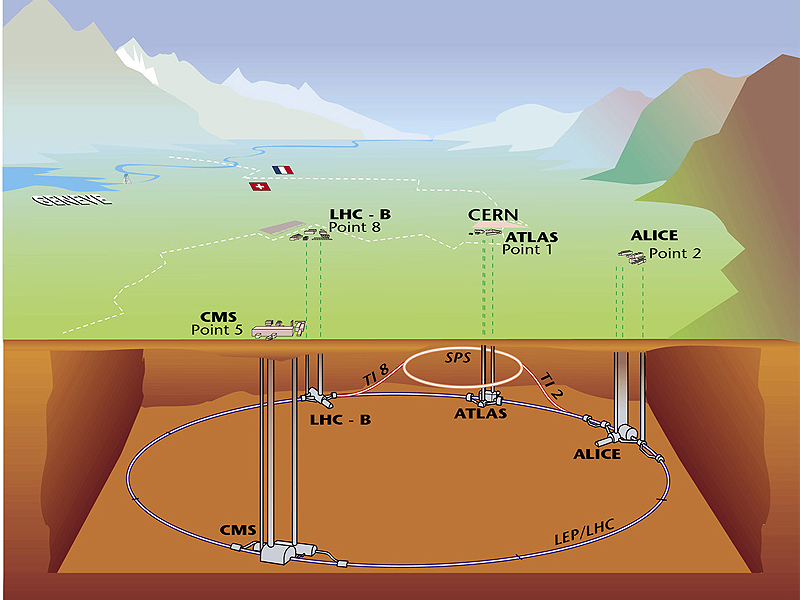
\includegraphics[width=9cm,height=6cm]{_figs/cernring-l.jpg}
\end{center}

\end{figure}

	\begin{block}{}
		The Large Hadron Collider (LHC).\\
A proton-proton collider of 27km of circumference.
	\end{block}{}


\end{frame}

\begin{frame}[fragile]
\frametitle{ATLAS installation}


\begin{figure}[h]
\begin{center}
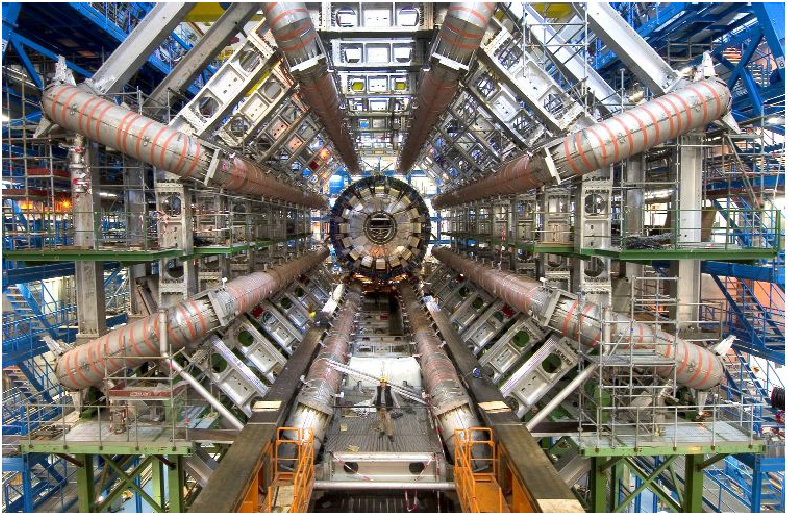
\includegraphics[width=10cm,height=7cm]{_figs/ATLAS-pit.png}
\end{center}

\end{figure}


\end{frame}

\begin{frame}[fragile]
	\begin{columns}
		\begin{column}{0.70\textwidth}
			\begin{block}{}
				\begin{center}
(a brief) History of software in HEP
				\end{center}
			\end{block}
		\end{column}
	\end{columns}




\end{frame}

\begin{frame}[fragile]
\frametitle{50's-90's: FORTRAN77}

	\begin{block}{}
\begin{minted}[]{fortran}
c     == hello.f ==
      program main
      implicit none
      write ( *, '(a)' ) 'Hello from FORTRAN'
      stop
      end
\end{minted}
	\end{block}{}


	\begin{exampleblock}{}
\begin{verbatim}
$ gfortran -c hello.f && gfortran -o hello hello.o
$ ./hello
Hello from FORTRAN
\end{verbatim}
	\end{exampleblock}{}


\begin{itemize}
\item \texttt{FORTRAN77} is the \textbf{king}
\item 1964: \textbf{CERNLIB}
\item REAP (paper tape measurements), THRESH (geometry reconstruction)
\item SUMX, \textbf{HBOOK} (statistical analysis chain)
\item ZEBRA (memory management, I/O, ...)
\item GEANT3, \textbf{PAW}
\end{itemize}


\end{frame}

\begin{frame}[fragile]
\frametitle{90's-...: C++}


	\begin{block}{}
\begin{minted}[]{cpp}
#include <iostream>
int main(int, char **) {
  std::cout << "Hello from C++" << std::endl;
  return EXIT_SUCCESS;
}
\end{minted}
	\end{block}{}


	\begin{exampleblock}{}
\begin{verbatim}
$ c++ -o hello hello.cxx && ./hello
Hello from C++
\end{verbatim}
	\end{exampleblock}{}


\begin{figure}[h]
\begin{center}

\includegraphics[width=2cm,height=2cm]{_figs/my-root6splash.png}
\end{center}

\end{figure}

\begin{itemize}
\item object-oriented programming (OOP) is the cool kid on the block
\item \textbf{ROOT}, POOL, LHC++, AIDA, \textbf{Geant4}
\item \texttt{C++} takes roots in HEP
\end{itemize}


\end{frame}

\begin{frame}[fragile]
\frametitle{00's-...: python}


	\begin{block}{}
\begin{minted}[]{py}
print "Hello from python"
\end{minted}
	\end{block}{}

	\begin{exampleblock}{}
\begin{verbatim}
$ python ./hello.py
Hello from python
\end{verbatim}
	\end{exampleblock}{}


\begin{figure}[h]
\begin{center}

\includegraphics[width=3cm,height=1cm]{_figs/my-python-logo.png}
\end{center}

\end{figure}

\begin{itemize}
\item \texttt{python} becomes the \emph{de} \emph{facto} scripting language in HEP
\item framework data-cards
\item analysis glue, (whole) analyses in \texttt{python}
\item \textbf{PyROOT}, rootpy
\item numpy, scipy, matplotlib, \textbf{IPython/Jupyter}
\end{itemize}


\end{frame}

\begin{frame}[fragile]
\frametitle{Current software in a nutshell}


\begin{itemize}
\item \textbf{Generators}: generation of true particles from fondamental physics first principles
\item \textbf{Full} \textbf{Simulation}: tracking of all stable particles in magnetic field through the detector simulating interaction, recording energy deposition (\textbf{CPU} \textbf{intensive})
\item \textbf{Reconstruction}: from real data, or from \texttt{Monte-Carlo} simulation data as above
\item \textbf{Fast} \textbf{Simulation}: parametric simulation, faster, coarser
\item \textbf{Analysis}: daily work of physicists, running on output of reconstruction to derive analysis specific information (\textbf{I/O} \textbf{intensive})
\item everything in the same \texttt{C++} offline control framework (except analysis)
\end{itemize}

\begin{figure}[h]
\begin{center}
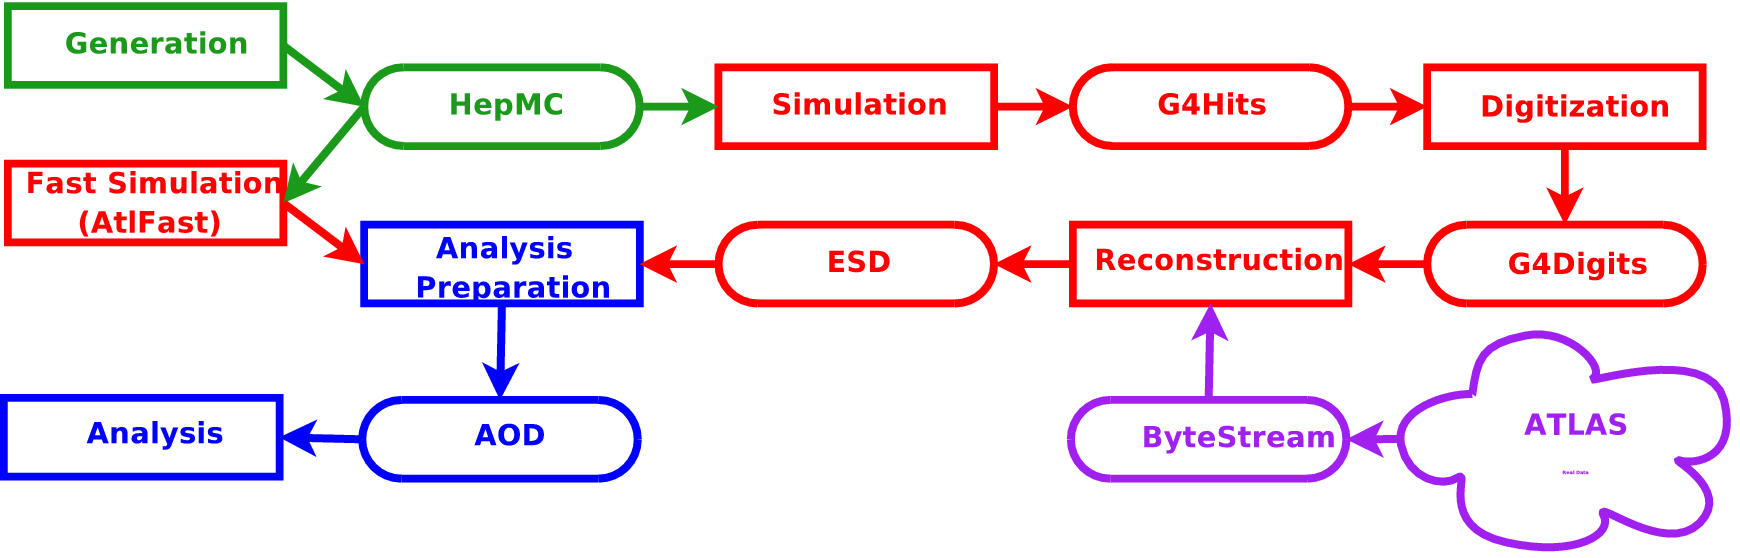
\includegraphics[width=\textwidth]{_figs/data-flux-summary-all.png}
\end{center}

\end{figure}


\end{frame}

\begin{frame}[fragile]
\frametitle{Software in HEP - some numbers}

	\begin{exampleblock}{}
		An LHC experiment (\emph{e.g.} \texttt{ATLAS}, \texttt{CMS}) is about $\sim$3000 physicists large but only a fraction of those is developing code.


Reconstruction frameworks grew from $\sim$3M SLOC to $\sim$5M
	\end{exampleblock}{}

	\begin{block}{}
Summing over all HEP software stack for \emph{e.g.} ATLAS:


\begin{itemize}
\item event generators: $\sim$1.4M SLOC (C++, FORTRAN-77)
\item I/O libraries $\sim$1.7M SLOC (C++)
\item simulation libraries $\sim$1.2M SLOC (C++)
\item reconstruction framework $\sim$5M SLOC (C++) + steering/configuration ($\sim$1M SLOC python) (want to have a look at the \myblue{\href{http://acode-browser.usatlas.bnl.gov/lxr/source/}{\texttt{ATLAS code}}}? \myblue{\href{https://github.com/cms-sw/cmssw}{\texttt{CMS code}}}?)
\end{itemize}
	\end{block}{}

\textbf{GCC:} $\sim$7M SLOC


\textbf{Linux} \textbf{kernel} \textbf{3.6:} 15.9M SLOC



\end{frame}

\begin{frame}[fragile]
\frametitle{People committing code to VCS per month}


	\begin{exampleblock}{}
		\begin{itemize}
	\item Variety of skills\\
	\item Huge turn-around\\
	\item Once the physics data is pouring, people go doing physics instead of software\\
		\end{itemize}
	\end{exampleblock}{}
	

\begin{figure}[h]
\begin{center}
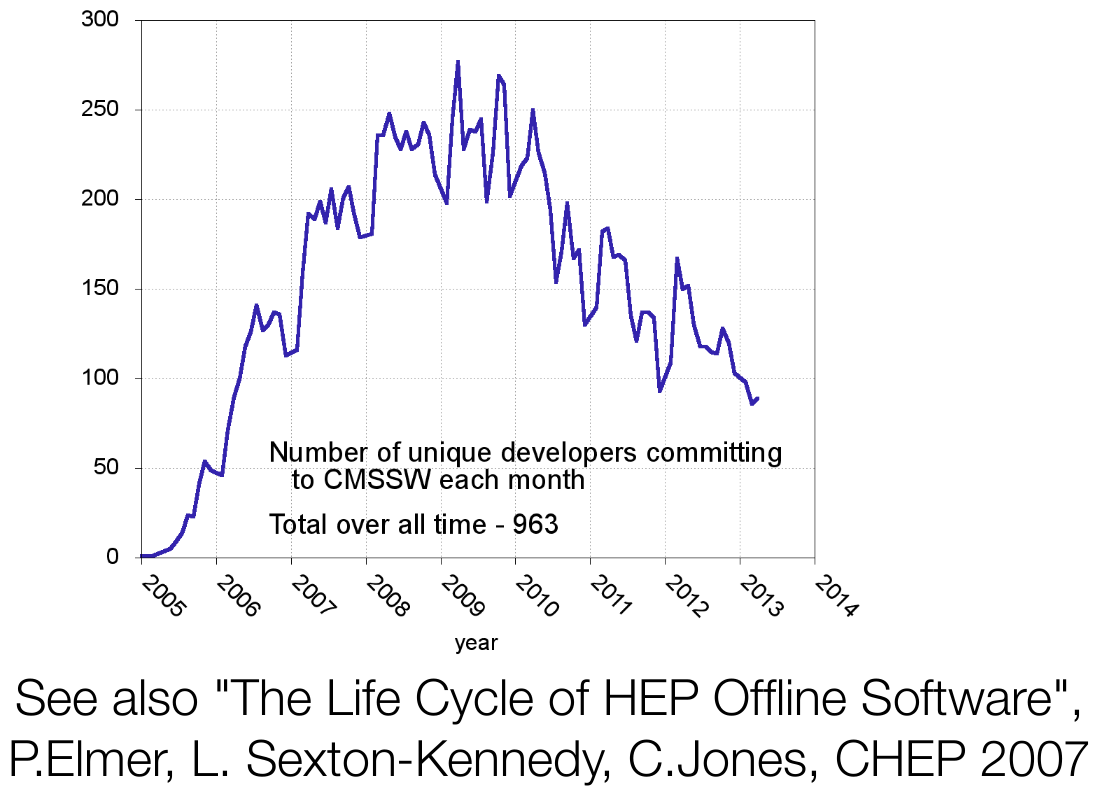
\includegraphics[width=8cm,height=5cm]{_figs/cmssw-commits.png}
\end{center}

\end{figure}


\end{frame}

\begin{frame}[fragile]
\frametitle{Software developers}


	\begin{block}{}
$\sim$300 active developers (per experiment)


$\sim$1000 different developers integrated over the lifetime of a single LHC experiment.


\begin{itemize}
\item few "real" s/w experts
\item some physicists with strong skill set in s/w
\item many with some experience in s/w development
\item some with \textbf{no} experience in s/w development
\end{itemize}
	\end{block}{}

\qquad\\
A multi-timezone environment


\begin{itemize}
\item Europe, America, Asia, Australia
\end{itemize}

Many communities (core s/w people, generators, simulation, ...)


\qquad\\

Development and infrastructures usually CERN-centric

Heavily Linux based (\myblue{\href{http://linux.web.cern.ch/linux/centos7/}{\texttt{Scientific Linux CERN}}}, \myblue{\href{https://linux.web.cern.ch/linux/centos7/}{\texttt{CERN CentOS}}})



\end{frame}

\begin{frame}[fragile]
\frametitle{Software development cycle}


VCS (CVS, then SVN. GIT: getting there.)


	\begin{block}{}
Nightlies (Jenkins, Travis or homegrown solution)


\begin{itemize}
\item need a sizeable cluster of build machines (distcc, ccache, ...)
\item builds the framework stack in $\sim$8h
\item produces $\sim$2000 shared libraries
\item installs them on AFS (also creates RPMs and tarballs)
\end{itemize}

Devs can then test and develop off the nightly \emph{via} AFS

	\end{block}{}

	Every 6 months or so a new production release is cut, validated (then patched) and deployed on the World Wide LHC Computing Grid (\myblue{\href{http://wlcg.web.cern.ch/}{\texttt{WLCG}}}).


	\begin{block}{}
Release size: \textbf{$\sim$5Gb}


\begin{itemize}
\item binaries, libraries (externals+framework stack)
\item extra data (sqlite files, physics processes' modelisation data, ...)
\end{itemize}

	\end{block}{}

\end{frame}

\begin{frame}[fragile]
\frametitle{Software runtime ?}


	\emph{Big science, big data, big software, big numbers.}

	\begin{block}{}
\begin{itemize}
\item $\sim$1min to initialize the application
\item loading $>$500 shared libraries
\item connecting to databases (detector description, geometry, ...)
\item instantiating $\sim$2000 \texttt{C++} components (steered from a \texttt{Python} script)
\item 2Gb/4Gb memory footprint per process
\end{itemize}
	\end{block}{}

\end{frame}

\begin{frame}[fragile]
\frametitle{(obligatory xkcd reference)}


\begin{itemize}
\item \texttt{C++}: \textbf{slow} (very slow?) to compile/develop, \textbf{fast} to execute
\item \texttt{python}: \textbf{fast} development cycle (no compilation), \textbf{slow} to execute
\end{itemize}

\begin{figure}[h]
\begin{center}
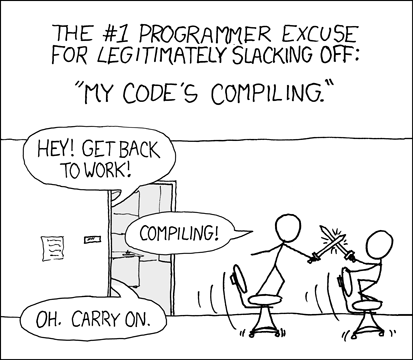
\includegraphics[width=5cm,height=5cm]{_figs/xkcd-compiling.png}
\end{center}

\end{figure}


\end{frame}

\begin{frame}[fragile]
\frametitle{}


	We learn to love hating our framework. \emph{(every step of the way)}

	\begin{block}{}
And even more so in the future:


\begin{itemize}
\item work to make our software stack thread-safe
\item or at least parts of it multithread friendly to harness multicore machines
\item quite a lot of fun ahead
\end{itemize}
	\end{block}{}

\end{frame}

\begin{frame}[fragile]
\frametitle{Other software engineering problems}

	\begin{block}{}
\begin{itemize}
\item scalability (development, teaching, maintenance, build)
\item installation of dependencies
\item code deployment
\item code robustness
\item code readability
\item multicores/manycores, multithreading
\item distributed programming
\item etc...
\end{itemize}
	\end{block}{}

	\quad\\

\myblue{\href{https://talks.golang.org/2012/splash.slide}{\texttt{talks.golang.org/2012/splash.slide}}}

\myblue{\href{https://talks.golang.org/2012/splash.article}{\texttt{talks.golang.org/2012/splash.article}}}


\end{frame}

\begin{frame}[fragile]
\frametitle{Are those our only options ?}


\begin{figure}[h]
\begin{center}
\includegraphics[width=11cm,height=6cm]{_figs/funfast-nogo_svg.png}
\end{center}

\caption{Credits: B. Fitzpatrick}

\end{figure}


\end{frame}

\begin{frame}[fragile]
\frametitle{Remember Go ?}


\begin{itemize}
\item compiles quickly (no warnings, imports)
\item enforces coherent coding rules (across projects)
\item builtin test/benchmark/documentation facilities
\item deploys easily, cross-compiles easily
\item installs easily (also 3rd-party packages: \texttt{go get})
\item fast to pick up, not as complicated as \textbf{C++}
\item builtin reflection system
\item builtin (de)serialization capabilities
\item concurrency support
\item garbage collected
\end{itemize}

\quad\\

	\begin{block}{}

		\textbf{Perfect} \textbf{match} for many HEP use cases.

	\end{block}{}


\end{frame}

\begin{frame}[fragile]
\frametitle{Migrating to Go ? (evil plan for (HEP) world domination)}


Migrating $\sim$5M SLOC of C++ code to Go, during data taking, \textbf{unfortunately}, won't fly.

\quad\\

Creating new applications for data massaging or post-processing \textbf{might}.


Creating a new concurrent and parallel framework for the next accelerator \textbf{might}.

\quad\\

	\begin{columns}
		\begin{column}{0.70\textwidth}
	\begin{block}{}
Need to build a critical mass of Go HEP enthusiasts
	\end{block}{}
		\end{column}
	\end{columns}


\end{frame}

\begin{frame}[fragile]
	\begin{columns}
		\begin{column}{0.49\textwidth}
			\begin{block}{}
				\begin{center}
Go-HEP
				\end{center}
			\end{block}
		\end{column}
	\end{columns}



\end{frame}

\begin{frame}[fragile]
\frametitle{What can Go bring to science and HEP?}


\begin{itemize}
\item a \textbf{simple} language anybody can learn in days, proficient in a couple of months
\item \textbf{standard} tool to handle \textbf{dependencies} (across OSes, architectures)
\item \textbf{fast} edit-compile-run development cycle
\item \textbf{simple} deployment (on clusters, laptops, ...), \textbf{easiest} \textbf{cross-compilation} system to date
\item fast at runtime, builtin tools for profiling (CPU, mem, flamegraph, tracing)
\item support for \textbf{concurrency} programming and multi-core machines
\item no magic, no voodoo, \textbf{reduce} disconnect b/w HEP sw experts and HEP users
\item \textbf{easy} code sharing: between packages, between experiments, between scientists
\item easier \textbf{reproducibility} and cross-check tests
\item \textbf{refactoring} tools \& linters, builtin/standard testing tools
\end{itemize}

	\begin{block}{}
		\begin{center}
\myblue{\href{https://sbinet.github.io/posts/2018-07-31-go-hep-manifesto}{\texttt{sbinet.github.io/posts/2018-07-31-go-hep-manifesto}}}
		\end{center}
	\end{block}{}


\end{frame}

\begin{frame}[fragile]
\frametitle{Go for HEP: challenges}


\texttt{\$EXPERIMENT} is taking data:


\begin{itemize}
\item one can't really migrate (monolithic) MLoC software stacks while taking data, neither during a long shutdown
\end{itemize}

	\begin{block}{\textbf{Convincing} physicists:}


\begin{itemize}
\item need to prove \texttt{Go} is useful, pleasant to use and viable
\item need to prove one can carry an analysis in \texttt{Go}, faster than by other means
\item provide 1 or 2 "poster child" applications
\end{itemize}
	\end{block}{}

\textbf{Need} to implement:


\begin{itemize}
\item histograms, PDFs, plotting, fits, BLAS/LAPACK, I/O
\item (some level of) inter-operability with \texttt{C++/ROOT}
\end{itemize}

	\begin{block}{}
		\begin{center}
$\Rightarrow$ \myblue{\href{https://go-hep.org}{\texttt{go-hep.org}}} is the beginning of such an endeavour
		\end{center}
	\end{block}{}


\end{frame}

\begin{frame}[fragile]
	\frametitle{\texttt{https://go-hep.org}}


\begin{figure}[h]
\begin{center}
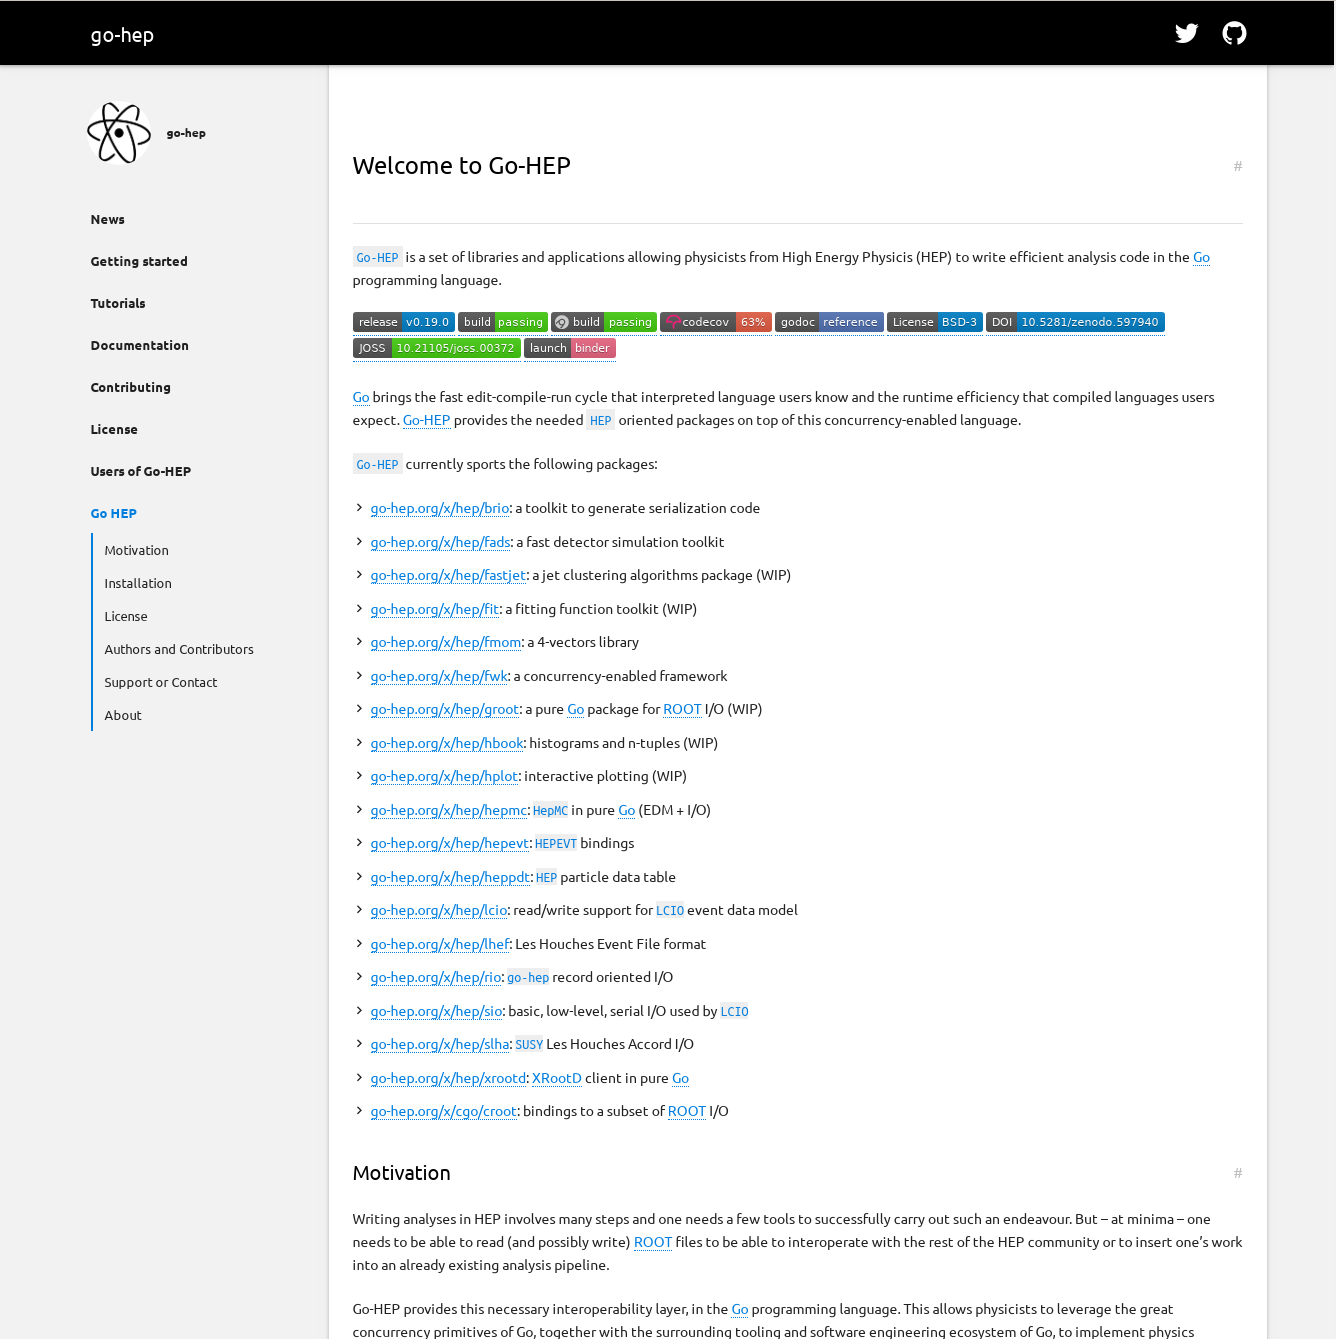
\includegraphics[width=8cm,height=8cm]{_figs/go-hep-home.png}
\end{center}

\end{figure}


\end{frame}

\begin{frame}[fragile]
\frametitle{}


Available and tested (TravisCI, AppVeyor) on Windows, Linux, Darwin, ... AMD64, 386, ARM, ARM64, ...


\begin{itemize}
\item \myblue{\href{https://go-hep.org/x/hep/brio}{\texttt{go-hep.org/x/hep/brio}}}: a toolkit to generate serialization code
\item \myblue{\href{https://go-hep.org/x/hep/fads}{\texttt{go-hep.org/x/hep/fads}}}: a fast detector simulation toolkit
\item \myblue{\href{https://go-hep.org/x/hep/fastjet}{\texttt{go-hep.org/x/hep/fastjet}}}: a jet clustering algorithms package (WIP)
\item \myblue{\href{https://go-hep.org/x/hep/fit}{\texttt{go-hep.org/x/hep/fit}}}: a fitting function toolkit (WIP)
\item \myblue{\href{https://go-hep.org/x/hep/fmom}{\texttt{go-hep.org/x/hep/fmom}}}: a 4-vectors library
\item \myblue{\href{https://go-hep.org/x/hep/fwk}{\texttt{go-hep.org/x/hep/fwk}}}: a concurrency-enabled control framework
\item \myblue{\href{https://go-hep.org/x/hep/hbook}{\texttt{go-hep.org/x/hep/hbook}}}: histograms and n-tuples (WIP)
\item \myblue{\href{https://go-hep.org/x/hep/hplot}{\texttt{go-hep.org/x/hep/hplot}}}: interactive plotting (WIP)
\item \emph{[...]}
\item \myblue{\href{https://go-hep.org/x/hep/groot}{\texttt{go-hep.org/x/hep/groot}}}: a pure \myblue{\href{https://golang.org}{\texttt{Go}}} package to for \myblue{\href{https://root.cern.ch}{\texttt{ROOT}}} I/O
\item \myblue{\href{https://go-hep.org/x/hep/xrootd}{\texttt{go-hep.org/x/hep/xrootd}}}: \myblue{\href{http://xrootd.org}{\texttt{XRootD}}} client in pure \myblue{\href{https://golang.org}{\texttt{Go}}}
\end{itemize}


\end{frame}

\begin{frame}[fragile]
\frametitle{Go-HEP}


	\begin{block}{}
\myblue{\href{https://doi.org/10.5281/zenodo.597940}{\texttt{DOI:10.5281 (Zenodo:597940)}}}

\myblue{\href{http://joss.theoj.org/papers/0b007c81073186f7c61f95ea26ad7971}{\texttt{JOSS Paper}}}
	\end{block}{}
	\quad\\

2 work areas to demonstrate `Go`'s applicability for HEP use cases have been identified:


\begin{itemize}
\item data acquisition (\texttt{DAQ}), monitoring, control command
\item detector fast simulation toolkit (\`a la \myblue{\href{https://cp3.irmp.ucl.ac.be/projects/delphes}{\texttt{Delphes (C++)}}})
\end{itemize}


\end{frame}

\begin{frame}[fragile]
	\begin{columns}
		\begin{column}{0.70\textwidth}
			\begin{block}{}
				\begin{center}
Go-HEP - fast-simulation \& analysis
				\end{center}
			\end{block}
		\end{column}
	\end{columns}



\end{frame}

\begin{frame}[fragile]
\frametitle{fads}


\texttt{fads} is a "FAst Detector Simulation" toolkit.


\begin{itemize}
\item morally a translation of \myblue{\href{https://cp3.irmp.ucl.ac.be/projects/delphes}{\texttt{C++-Delphes}}} into Go
\item uses \myblue{\href{https://go-hep.org/x/hep/fwk}{\texttt{hep/fwk}}} to expose, manage and harness concurrency into the usual \texttt{HEP} event loop (\texttt{initialize} | \texttt{process-events} | \texttt{finalize})
\item uses \myblue{\href{https://go-hep.org/x/hep/hbook}{\texttt{hep/hbook}}} for histogramming, \myblue{\href{htpps://go-hep.org/x/hep/hepmc}{\texttt{hep/hepmc}}} for \texttt{HepMC} input/output
\end{itemize}

	\begin{block}{}
Code is on github (BSD-3):


\myblue{\href{https://go-hep.org/x/hep/fwk}{\texttt{go-hep.org/x/hep/fwk}}}

\myblue{\href{https://go-hep.org/x/hep/fads}{\texttt{go-hep.org/x/hep/fads}}}
	\end{block}{}

	\begin{exampleblock}{}
Documentation is served by \myblue{\href{https://godoc.org}{\texttt{godoc.org}}}:


\myblue{\href{https://godoc.org/go-hep.org/x/hep/fwk}{\texttt{godoc.org/go-hep.org/x/hep/fwk}}}

\myblue{\href{https://godoc.org/go-hep.org/x/hep/fads}{\texttt{godoc.org/go-hep.org/x/hep/fads}}}

	\end{exampleblock}{}

\end{frame}

\begin{frame}[fragile]
\frametitle{go-hep/fwk}


\myblue{\href{https://go-hep.org/x/hep/fwk}{\texttt{fwk}}} is a Go-based concurrent control framework inspired from:


\begin{itemize}
\item GaudiHive
\item ILC Marlin
\item CMSSW
\item previous incarnations of \emph{fwk} (\emph{go-ng-gaudi}, \emph{go-gaudi})
\end{itemize}


\end{frame}

\begin{frame}[fragile]
\frametitle{go-hep/fwk - Examples}


	\begin{block}{}
\begin{verbatim}
$ fwk-ex-tuto-1 -help
Usage: fwk-ex-tuto1 [options]

ex:
 $ fwk-ex-tuto-1 -l=INFO -evtmax=-1

options:
  -evtmax=10: number of events to process
  -l="INFO": message level (DEBUG|INFO|WARN|ERROR)
  -nprocs=0: number of events to process concurrently

\end{verbatim}
	\end{block}{}


Runs 2 tasks.


\begin{figure}[h]
\begin{center}
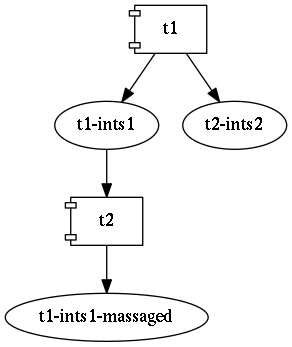
\includegraphics[width=2cm,height=2cm]{_figs/fwk-ex1-dflow.png}
\end{center}

\end{figure}


\end{frame}

\begin{frame}[fragile]

\begin{minted}[]{sh}
$ fwk-ex-tuto-1
::: fwk-ex-tuto-1...
t2                   INFO configure...
t2                   INFO configure... [done]
t1                   INFO configure ...
t1                   INFO configure ... [done]
t2                   INFO start...
t1                   INFO start...
app                  INFO >>> running evt=0...
t1                   INFO proc... (id=0|0) => [10, 20]
t2                   INFO proc... (id=0|0) => [10 -> 100]
[...]
app                  INFO >>> running evt=9...
t1                   INFO proc... (id=9|0) => [10, 20]
t2                   INFO proc... (id=9|0) => [10 -> 100]
t2                   INFO stop...
t1                   INFO stop...
app                  INFO cpu: 654.064us
app                  INFO mem: alloc:             62 kB
app                  INFO mem: tot-alloc:         74 kB
::: fwk-ex-tuto-1... [done] (cpu=788.578us)

\end{minted}


\end{frame}

\begin{frame}[fragile]
\frametitle{go-hep/fwk - Components}


A \texttt{fwk} application consists of a set of components (\texttt{fwk.Task}) which are:


\begin{itemize}
\item (optionally) configured
\item started
\item given the chance to process each event
\item stopped
\end{itemize}

Helper components (\texttt{fwk.Svc}) can provide additional features (such as a whiteboard/event-store service, a data-flow service, ...) but do not typically take (directly) part of the event processing.



\end{frame}

\begin{frame}[fragile]
\frametitle{go-hep/fwk - Interfaces}


\begin{minted}[]{go}
// Component is the interface satisfied by all values in fwk.
//
// A component can be asked for:
// its Type() (ex: "go-hep.org/x/hep/fads.MomentumSmearing")
// its Name() (ex: "MuonsMomSmearing")
type Component interface {
	Type() string
	Name() string
}
\end{minted}

\texttt{Tasks} (and \texttt{Services}) are called with a \texttt{Context} argument to enable concurrency/parallelism.


\begin{minted}[]{go}
// Task is a component processing event-level data.
// Task.Process is called for every component and for every input event.
type Task interface {
	Component

	StartTask(ctx Context) error
	Process(ctx Context) error
	StopTask(ctx Context) error
}
\end{minted}


\end{frame}

\begin{frame}[fragile]
\frametitle{go-hep/fwk - Interfaces}


\begin{minted}[]{go}
// Context is the interface to access context-local data.
type Context interface {
	ID() int64      // id of this context (e.g. entry/event number)
	Slot() int      // slot number in the pool of event sequences
	Store() Store   // data store corresponding to the id+slot
	Msg() MsgStream // messaging for this context (id+slot)

	// Svc retrieves an already existing Svc by name.
	Svc(n string) (Svc, error)
}

\end{minted}

\texttt{Context} is a bit of a grab bag of what needs to be available/queried during event processing.


\begin{itemize}
\item \texttt{Msg()} allows to relieve pressure on the I/O system. Eventually, should allow to have human-readable log files even with many events in-flight.
\end{itemize}

\begin{itemize}
\item similarly, \texttt{Store()} and \texttt{Svc()} allow to have event-level local state.
\end{itemize}


\end{frame}

\begin{frame}[fragile]
\frametitle{go-hep/fwk - Interfaces}


\begin{minted}[]{go}
// DeclPorter is the interface to declare in/out ports for the data flow.
type DeclPorter interface {
	DeclInPort(name string, t reflect.Type) error
	DeclOutPort(name string, t reflect.Type) error
}

\end{minted}

\begin{itemize}
\item Note there is no \emph{update} nor \emph{R/W} ports: simplifies the data flow, make it more \textbf{functional-like},
\item Updates handled by copying input data under a new event store key,
\item The \texttt{dflowsvc} detects (long-range) cycles and missing data-nodes.
\end{itemize}

\begin{minted}[highlightlines={2}]{go}
func (tsk *task1) Configure(ctx fwk.Context) error {
	err := tsk.DeclOutPort(tsk.i1prop, reflect.TypeOf(int64(0)))
	if err != nil {
		return xerrors.Errorf(
			"could not declare output port: %w", err,
		)
	}
	// ...
	return err
}

\end{minted}


\end{frame}

\begin{frame}[fragile]
\frametitle{go-hep/fwk - Interfaces}


\begin{minted}[]{go}
// Store provides access to a goroutine-safe map[string]interface{} store.
type Store interface {
	Get(key string) (interface{}, error)
	Put(key string, value interface{}) error
	Has(key string) bool
}

\end{minted}

Examples:


\begin{minted}[highlightlines={4,10}]{go}
func (tsk *task2) Process(ctx fwk.Context) error {
	store := ctx.Store()
	// blocks until data for this event/slot is available
	v, err := store.Get(tsk.input)
	if err != nil {
		return err
	}
	i := v.(int64)
	o := tsk.fct(i)
	err = store.Put(tsk.output, o)
	return err
}

\end{minted}


\end{frame}

\begin{frame}[fragile]
\frametitle{go-hep/fwk - appmgr}


\begin{minted}[highlightlines={8,10}]{go}
func (app *appmgr) run(ctx Context) error {
	var err error
	defer app.msg.flush()
	app.state = fsm.Running

	switch app.nprocs {
	case 0:
		err = app.runSequential(ctx)
	default:
		err = app.runConcurrent(ctx)
	}

	return err
}

\end{minted}

\begin{itemize}
\item run sequentially
\item run \emph{N} workers, each worker processing events as they become available
\item all tasks are started at the beginning of the event processing, letting the dataflow works its magic
\end{itemize}


\end{frame}

\begin{frame}[fragile]
\frametitle{go-hep/fwk - workers}


\begin{minted}[]{go}
type worker struct {
	slot  int
	keys  []string // nodes in data-flow (Input/Output)
	store datastore
	ctxs  []context // a Context for each component
	msg   msgstream

	evts <-chan int64    // channel of event indices
	quit <-chan struct{} // channel to notify early-abort
	done chan<- struct{} // channel to notify we are done
	errc chan<- error    // channel of errors during event processing
}

\end{minted}

\begin{itemize}
\item each worker manages its own event store
\item each worker manages contexts for each component it runs
\end{itemize}


\end{frame}

\begin{frame}[fragile]
\frametitle{go-hep/fwk - workers}


	\begin{block}{}
\myblue{\href{https://go-hep.org/x/hep/fwk}{\texttt{fwk}}} enables:


\begin{itemize}
\item event-level concurrency
\item tasks-level concurrency
\end{itemize}
	\end{block}{}

\myblue{\href{https://go-hep.org/x/hep/fwk}{\texttt{fwk}}} relies on \myblue{\href{https://golang.org}{\texttt{Go}}}'s runtime to properly schedule \emph{goroutines}.

\quad\\

For sub-task concurrency, users are by construction required to use \myblue{\href{https://golang.org}{\texttt{Go}}}'s constructs (\emph{goroutines} and \emph{channels}) so everything is consistent \textbf{and} the \emph{runtime} has the \textbf{complete} \textbf{picture}.



\end{frame}

\begin{frame}[fragile]
\frametitle{go-hep/fwk - configuration \& steering}


\begin{itemize}
\item use regular \myblue{\href{https://golang.org}{\texttt{Go}}} to configure and steer.
\item still on the fence on a DSL-based configuration language (\texttt{HCL}, \texttt{Toml}, ...)
\item probably \textbf{not} \texttt{Python} though
\end{itemize}

\begin{minted}[]{go}
// job is the scripting interface to 'fwk'
import "go-hep.org/x/hep/fwk/job"

func main() {
	// create a default fwk application, with some properties
	app := job.New(job.P{
		"EvtMax": 10,
		"NProcs": 2,
	})

	// ... cont'd on next page...

\end{minted}


\end{frame}

\begin{frame}[fragile]
\frametitle{}


\begin{minted}[]{go}
// create a task that reads integers from some location
// and publish the square of these integers under some other location
app.Create(job.C{
	Type: "go-hep.org/x/hep/fwk/testdata.task2",
	Name: "t2",
	Props: job.P{
		"Input":  "t1-ints1",
		"Output": "t1-ints1-massaged",
	},
})
// create a task that publish integers to some location(s)
app.Create(job.C{
	Type: "go-hep.org/x/hep/fwk/testdata.task1",
	Name: "t1",
	Props: job.P{
		"Ints1": "t1-ints1",
		"Ints2": "t2-ints2",
		"Int1":  int64(10), // initial value for the Ints1
		"Int2":  int64(20), // initial value for the Ints2
	},
})
app.Run()

\end{minted}


\end{frame}

\begin{frame}[fragile]
\frametitle{go-hep/fads - real world use case}


\begin{itemize}
\item translated \myblue{\href{https://cp3.irmp.ucl.ac.be/projects/delphes}{\texttt{C++-Delphes}}}' ATLAS data-card into Go
\item \myblue{\href{https://github.com/go-hep/hep/blob/master/fads/cmd/fads-app/main.go}{\texttt{go-hep/fads/cmd/fads-app}}}
\item installation:
\end{itemize}


	\begin{block}{}
\begin{verbatim}
$ go get go-hep.org/x/hep/fads/cmd/fads-app
$ fads-app -help
Usage: fads-app [options] <hepmc-input-file>

ex:
 $ fads-app -l=INFO -evtmax=-1 ./testdata/hepmc.data

options:
  -cpu-prof=false: enable CPU profiling
  -evtmax=-1: number of events to process
  -l="INFO": log level (DEBUG|INFO|WARN|ERROR)
  -nprocs=0: number of concurrent events to process

\end{verbatim}
	\end{block}{}


\end{frame}

\begin{frame}[fragile]
\frametitle{go-hep/fads - components}


\begin{itemize}
\item a \texttt{HepMC} converter
\item particle propagator
\item calorimeter simulator
\item energy rescaler, momentum smearer
\item isolation
\item b-tagging, tau-tagging
\item jet-finder (reimplementation of FastJet in Go: \myblue{\href{https://go-hep.org/x/hep/fastjet}{\texttt{go-hep/fastjet}}})
\item histogram service (from \myblue{\href{https://go-hep.org/x/hep/fwk}{\texttt{go-hep/fwk}}})
\end{itemize}

\end{frame}

\begin{frame}[fragile]
\frametitle{}


\begin{figure}[h]
\begin{center}
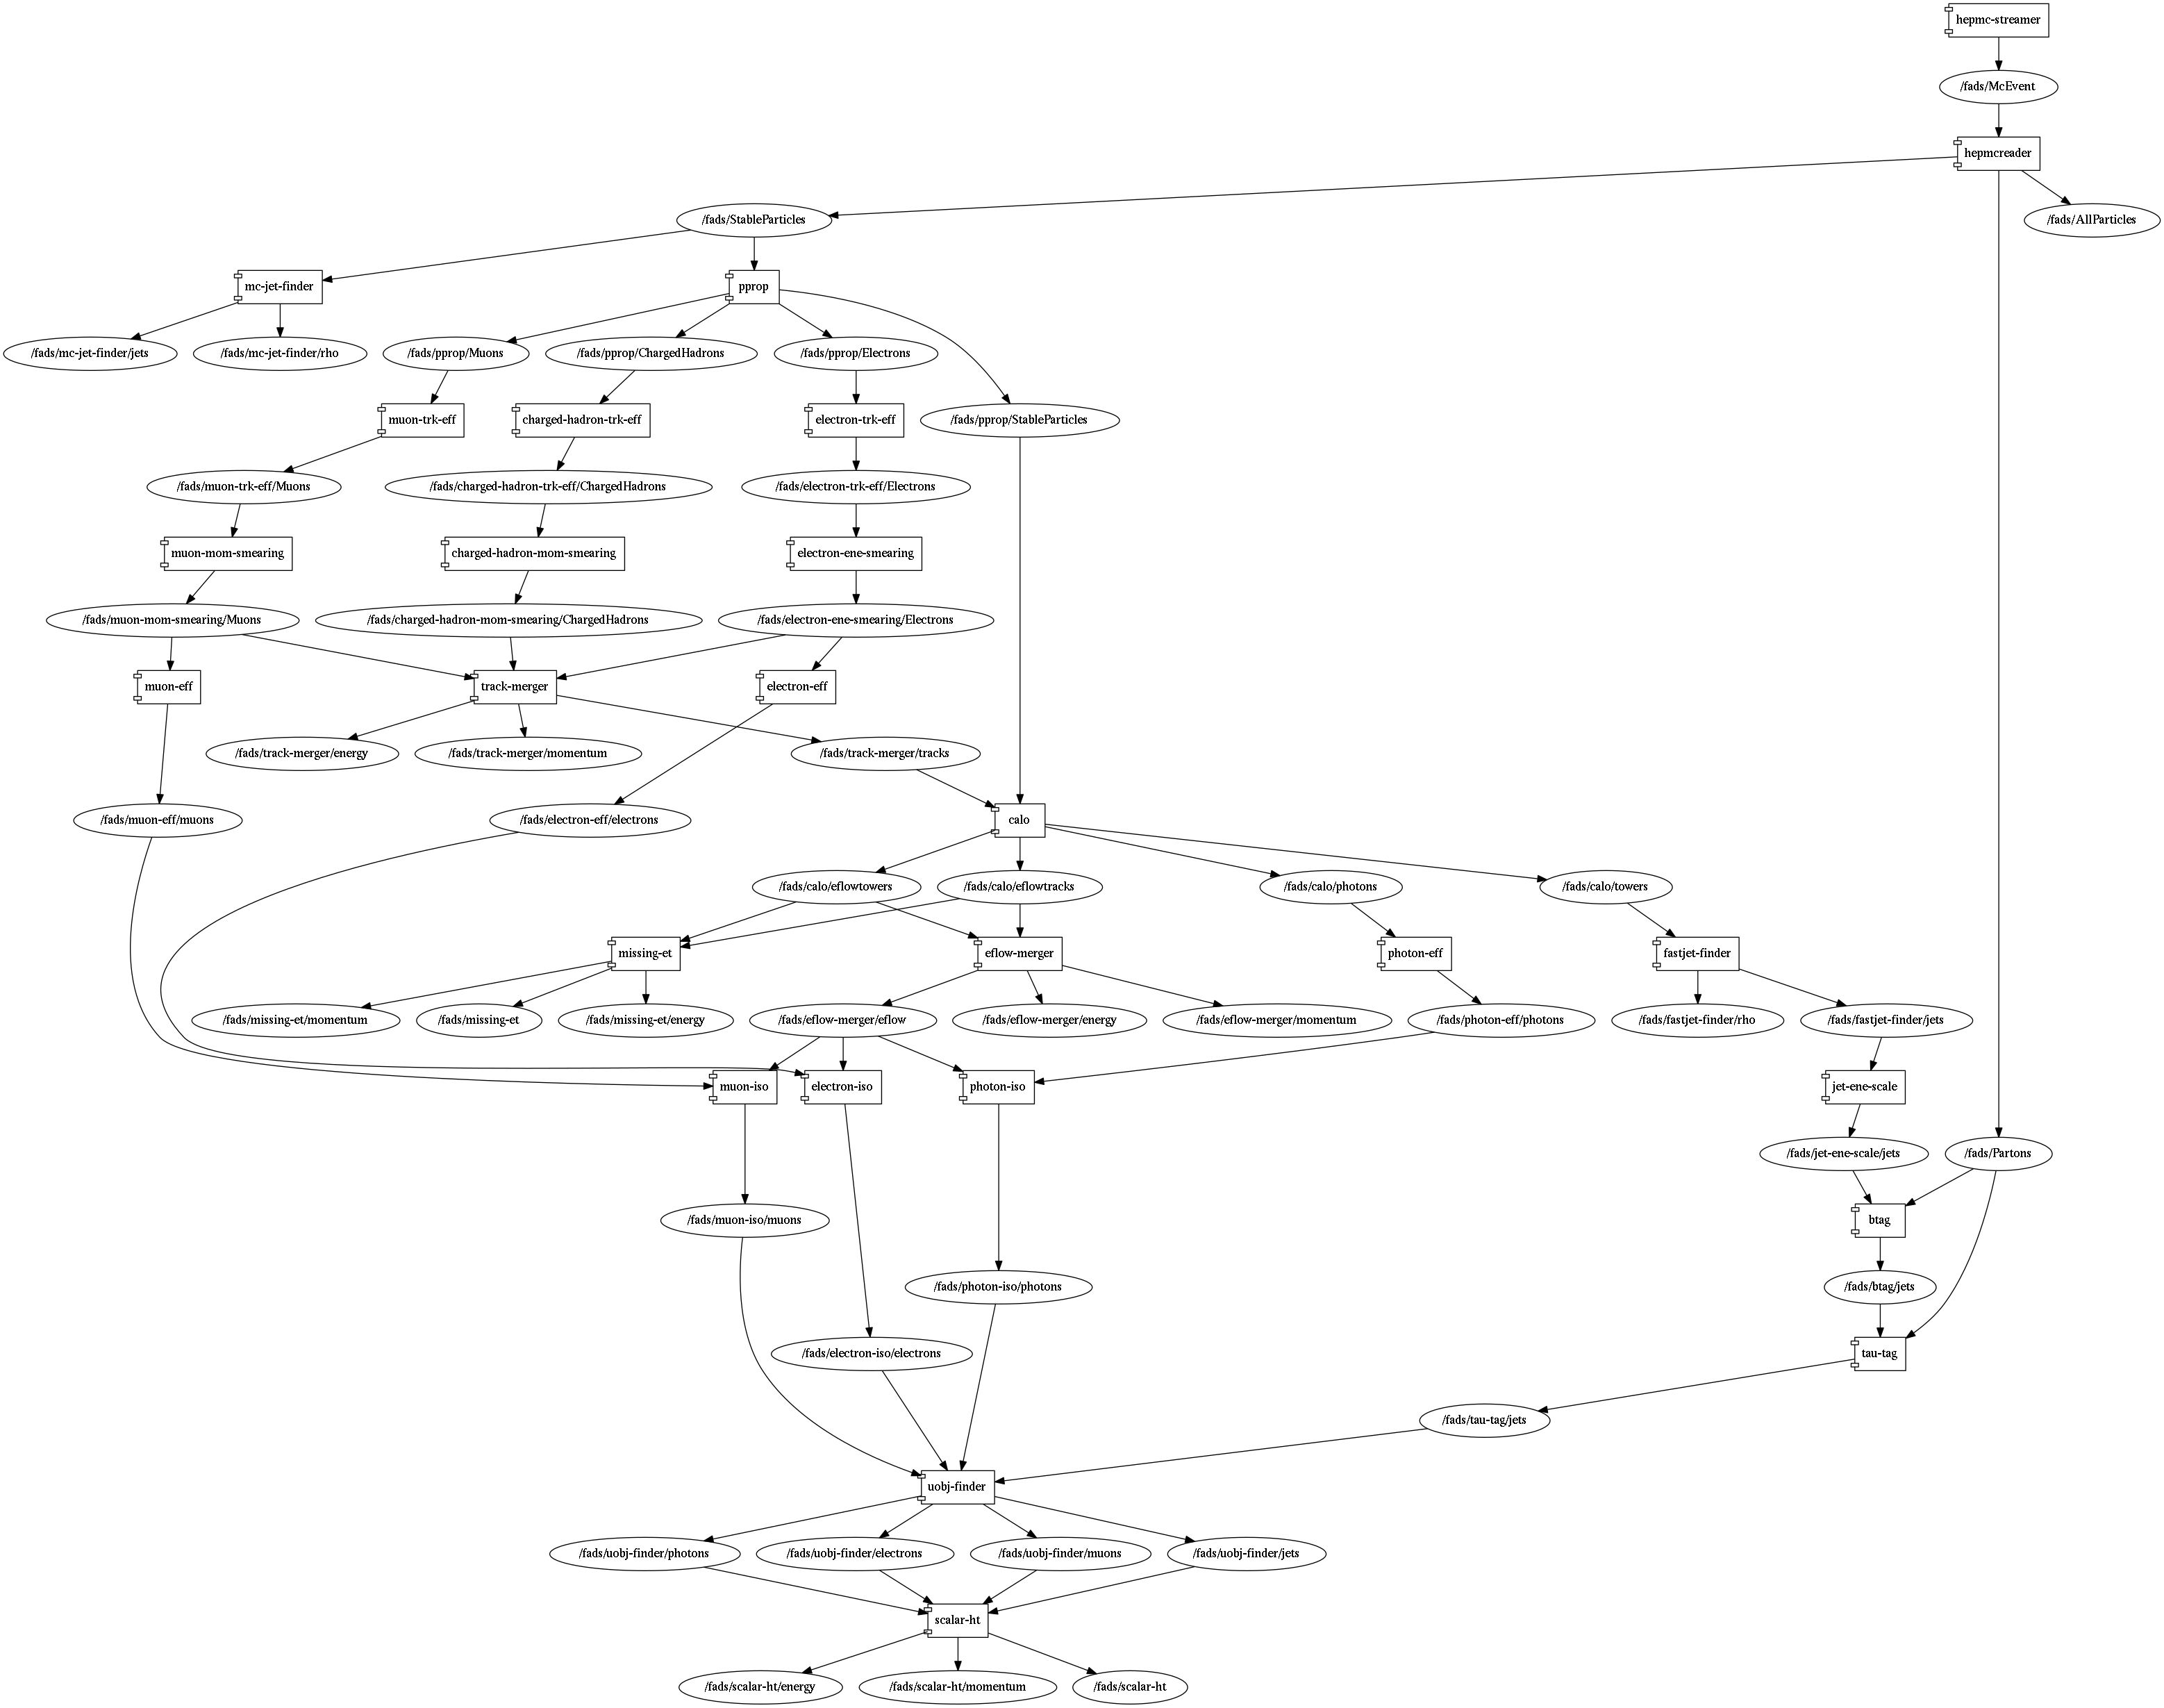
\includegraphics[width=8cm,height=8cm]{_figs/fads-dflow.png}
\end{center}

\end{figure}


\end{frame}

\begin{frame}[fragile]
\frametitle{Results - testbenches}


\begin{itemize}
\item Linux: Intel(R) Xeon(R) CPU E5-4620 0 @ 2.20GHz, 64 cores, 128Gb RAM
\end{itemize}

\begin{itemize}
\item Delphes, 3.0.12, gcc4.8
\item fads, Go-1.9
\end{itemize}

	\begin{block}{}
\begin{verbatim}
$> time delphes ./input.hepmc
$> time fads-app ./input.hepmc
\end{verbatim}
	\end{block}{}


\end{frame}

\begin{frame}[fragile]
\frametitle{}


\begin{figure}[h]
\begin{center}
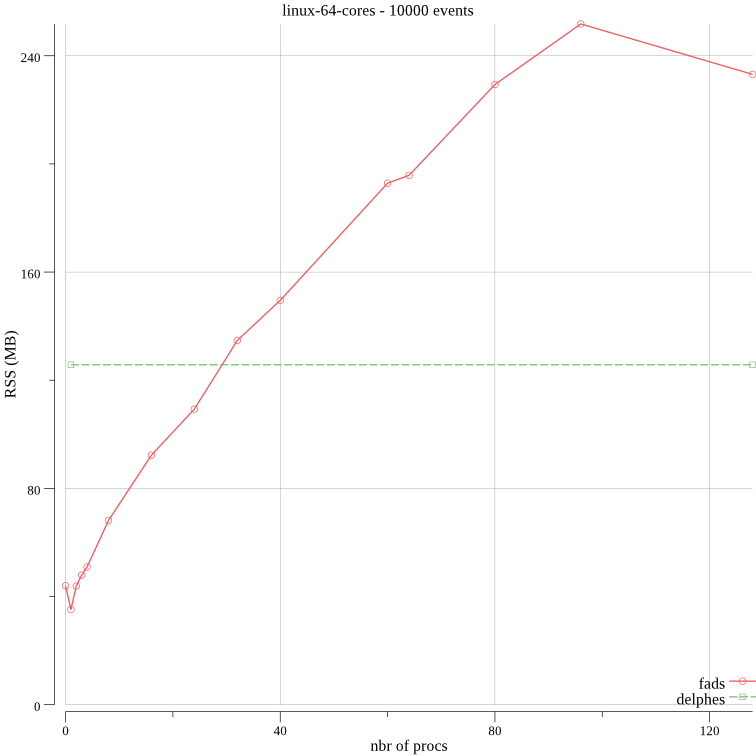
\includegraphics[width=8cm,height=8cm]{_figs/linux-64-cores-rss.png}
\end{center}

\end{figure}


\end{frame}

\begin{frame}[fragile]
\frametitle{}


\begin{figure}[h]
\begin{center}
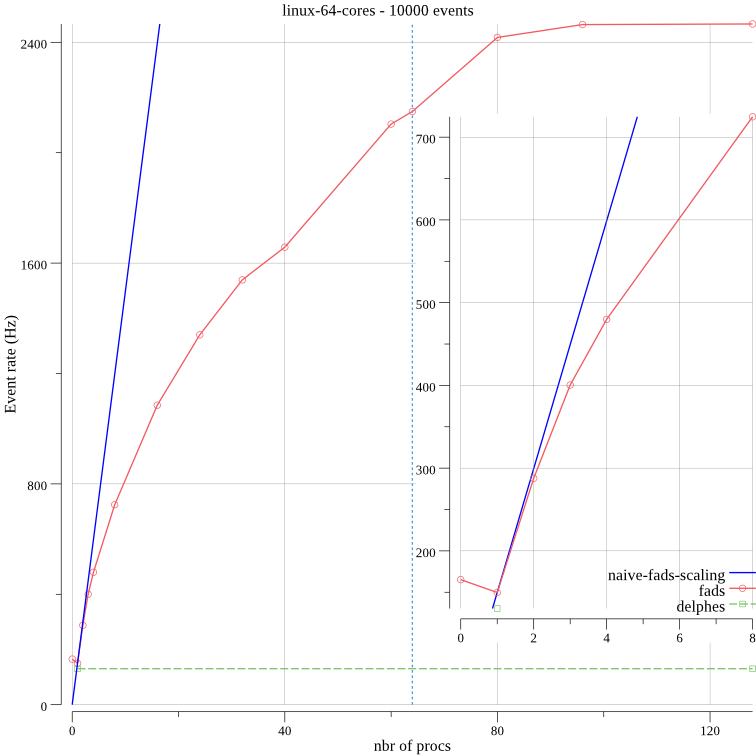
\includegraphics[width=8cm,height=8cm]{_figs/linux-64-cores-hz.png}
\end{center}

\end{figure}


\end{frame}

\begin{frame}[fragile]
\frametitle{fads: Results \& Conclusions}


\begin{itemize}
\item good RSS scaling
\item good CPU scaling
\end{itemize}

\begin{itemize}
	\item bit-by-bit matching physics results \emph{wrt} \texttt{Delphes}
	\item no need to merge output files, less chaotic I/O, less I/O wait
\end{itemize}


\end{frame}

\begin{frame}[fragile]
	\begin{columns}
		\begin{column}{0.70\textwidth}
			\begin{block}{}
				\begin{center}
Rivet \& fads
				\end{center}
			\end{block}
		\end{column}
	\end{columns}



\end{frame}

\begin{frame}[fragile]
\frametitle{Rivet}


The \myblue{\href{http://rivet.hepforge.org/}{\texttt{Rivet}}} toolkit (Robust Independent Validation of Experiment and Theory) is a system for validation of Monte Carlo event generators. It provides a large (and ever growing) set of experimental analyses useful for MC generator development, validation, and tuning, as well as a convenient infrastructure for adding your own analyses.


	\begin{block}{}
\begin{verbatim}
$> repeat 10 'time rivet --analysis=MC_GENERIC -q  ./Z-hadronic-LEP.hepmc'
real=13.32 user=12.97 sys=0.33 CPU=99% MaxRSS=26292
real=13.31 user=12.93 sys=0.37 CPU=99% MaxRSS=26356
real=13.29 user=12.93 sys=0.35 CPU=99% MaxRSS=26440
real=13.31 user=12.95 sys=0.35 CPU=99% MaxRSS=26356
real=13.29 user=13.01 sys=0.27 CPU=99% MaxRSS=26280
real=13.31 user=12.97 sys=0.32 CPU=99% MaxRSS=26328
real=13.35 user=12.93 sys=0.41 CPU=99% MaxRSS=26276
real=13.30 user=12.96 sys=0.33 CPU=99% MaxRSS=26624
real=13.30 user=12.93 sys=0.36 CPU=99% MaxRSS=26440
real=13.35 user=12.98 sys=0.36 CPU=99% MaxRSS=26484
\end{verbatim}
	\end{block}{}



\end{frame}

\begin{frame}[fragile]
\frametitle{fads-rivet-mc-generic}


Reimplementation on top of \myblue{\href{https://godoc.org/go-hep.org/x/hep/fwk}{\texttt{go-hep/fwk+fads}}} of the \texttt{MC\_GENERIC} analysis.


Bit-to-bit identical results.


	\begin{block}{}

\begin{verbatim}
$> go get go-hep.org/x/hep/fads/cmd/fads-rivet-mc-generic

$> repeat 10 'time fads-rivet-mc-generic -nprocs=1 ./Z-hadronic-LEP.hepmc'
real=6.04 user=5.66 sys=0.12 CPU= 95% MaxRSS=23384
real=5.70 user=5.62 sys=0.09 CPU=100% MaxRSS=21128
real=5.71 user=5.58 sys=0.11 CPU= 99% MaxRSS=22208
real=5.68 user=5.60 sys=0.08 CPU=100% MaxRSS=23156
real=5.71 user=5.63 sys=0.08 CPU=100% MaxRSS=20672
real=5.78 user=5.62 sys=0.09 CPU= 98% MaxRSS=22328
real=5.67 user=5.62 sys=0.05 CPU=100% MaxRSS=20968
real=5.68 user=5.57 sys=0.07 CPU= 99% MaxRSS=23748
real=5.70 user=5.60 sys=0.10 CPU=100% MaxRSS=21360
real=5.72 user=5.65 sys=0.07 CPU=100% MaxRSS=22764
\end{verbatim}
	\end{block}{}

	\begin{exampleblock}{}
		\begin{columns}
			\begin{column}{0.70\textwidth}
About 2x as fast, using a bit less memory.
			\end{column}
		\end{columns}
	\end{exampleblock}{}
\end{frame}


\begin{frame}[fragile]
	\begin{columns}
		\begin{column}{0.70\textwidth}
			\begin{block}{}
				\begin{center}
Go in science
				\end{center}
			\end{block}
		\end{column}
	\end{columns}


\end{frame}

\begin{frame}[fragile]
\frametitle{Science-y packages}


Even if \texttt{Go} is relatively new, support for general purpose scientific libraries is there and growing, thanks to the \myblue{\href{https://gonum.org}{\texttt{Gonum.org}}} community:


\begin{itemize}
\item \myblue{\href{https://godoc.org/gonum.org/v1/gonum/blas}{\texttt{gonum/blas}}}, a \texttt{Go} based implementation of Basic Linear Algebra Subprograms
\item \myblue{\href{https://godoc.org/gonum.org/v1/gonum/lapack}{\texttt{gonum/lapack}}}, a lapack implementation for \texttt{Go}
\item \myblue{\href{https://godoc.org/gonum.org/v1/gonum/mat}{\texttt{gonum/mat}}}, to work with matrices
\item \myblue{\href{https://godoc.org/gonum.org/v1/gonum/graph}{\texttt{gonum/graph}}}, to work with graphs
\item \myblue{\href{https://godoc.org/gonum.org/v1/gonum/optimize}{\texttt{gonum/optimize}}}, for finding the optimum value of functions
\item \myblue{\href{https://godoc.org/gonum.org/v1/gonum/integrate}{\texttt{gonum/integrate}}}, provides routines for numerical integration
\item \myblue{\href{https://godoc.org/gonum.org/v1/gonum/diff}{\texttt{gonum/diff}}}, for computing derivatives of a function
\item \myblue{\href{https://godoc.org/gonum.org/v1/gonum/stat}{\texttt{gonum/stat}}}, for statistics and distributions
\item \myblue{\href{http://godoc.org/gonum.org/v1/plot}{\texttt{gonum/plot}}}, to create publication quality plots (most of the plots seen earlier are made w/ \texttt{gonum/plot})
\item ...
\end{itemize}


\end{frame}

\begin{frame}[fragile]
\frametitle{I/O}


I/O support for some formats:


\begin{itemize}
\item \myblue{\href{https://github.com/sbinet/npyio}{\texttt{sbinet/npyio}}}: read/write support for \myblue{\href{http://docs.scipy.org/doc/numpy/neps/npy-format.html}{\texttt{NumPy data files}}}
\item \myblue{\href{https://github.com/ready-steady/mat}{\texttt{ready-steady/mat}}}, \myblue{\href{https://github.com/sbinet/matfio}{\texttt{sbinet/matfio}}}: r/w support for \myblue{\href{http://www.mathworks.com/help/pdf\_doc/matlab/apiext.pdf}{\texttt{MATLAB files}}}
\item \myblue{\href{https://github.com/gonum/hdf5}{\texttt{gonum/hdf5}}}: access to \myblue{\href{https://www.hdfgroup.org/HDF5}{\texttt{HDF5}}} (using \texttt{cgo})
\item \myblue{\href{https://godoc.org/github.com/apache/arrow/go/arrow}{\texttt{go-arrow}}}: access to \myblue{\href{https://arrow.apache.org}{\texttt{Apache Arrow}}} data and IPC protocol
\end{itemize}


\end{frame}

\begin{frame}[fragile]
\frametitle{Go for Data Science}


A data science community is gathering around \myblue{\href{https://gopherdata.io}{\texttt{gopherdata.io}}}.


\begin{itemize}
\item \myblue{\href{https://github.com/gopherdata/gophernotes}{\texttt{gopherdata/gophernotes}}}, a \myblue{\href{http://jupyter.org}{\texttt{Jupyter}}} kernel for \myblue{\href{https://golang.org}{\texttt{Go}}}
\item \myblue{\href{https://github.com/gopherdata/mybinder-go}{\texttt{gopherdata/mybinder-go}}}, a web-based Jupyter kernel for \myblue{\href{https://golang.org}{\texttt{Go}}}
\item \myblue{\href{https://github.com/gopherdata/resources/tree/master/tooling}{\texttt{gopherdata/resources}}}: many resources for machine learning, classifiers, neural networks, ...
\end{itemize}


\end{frame}

\begin{frame}[fragile]
\frametitle{Conclusions}


Go is great at writing small and large (concurrent) programs.
Also true for \textbf{science-y} programs, even if the amount of libraries can still be improved.


\begin{figure}[h]
\begin{center}
\includegraphics[width=7cm,height=4cm]{_figs/funfast_svg.png}
\end{center}

\end{figure}

Write your next tool/analysis/simulation/software in \myblue{\href{https://golang.org/}{\texttt{Go}}}? and \myblue{\href{https://go-hep.org}{\texttt{Go-HEP}}} or \myblue{\href{https://github.com/astrogo}{\texttt{astrogo}}}, or \myblue{\href{https://github.com/biogo}{\texttt{Biogo}}}, or \myblue{\href{https://gonum.org}{\texttt{Gonum}}}, or ...



\end{frame}

\begin{frame}[fragile]
\frametitle{Conclusions}


Go is great at writing small and large (concurrent) programs.
Also true for \textbf{science-y} programs, even if the amount of libraries can still be improved.


\begin{figure}[h]
\begin{center}
\includegraphics[width=7cm,height=4cm]{_figs/funfast_svg.png}
\end{center}
\end{figure}


	\begin{block}{}
\begin{verbatim}
Software engineering is what happens to programming
when you add time and other programmers.
(Russ Cox)
\end{verbatim}

		(Also true for science-y programs and scientists)
	\end{block}{}


\end{frame}

\begin{frame}[fragile]
\frametitle{Thank you}


\begin{figure}[h]
\begin{center}

\includegraphics[width=\textwidth]{logo-golab2019.png}
\end{center}
\end{figure}

	\begin{columns}
		\begin{column}{0.7\textwidth}
			\begin{block}{}
	\begin{columns}
		\begin{column}{0.2\textwidth}
\begin{figure}[h]
\begin{center}
\includegraphics[height=0.18\textheight]{_figs/avatar.png}
\end{center}
\end{figure}
		\end{column}

		\begin{column}{0.6\textwidth}
			\begin{center}
S\'ebastien Binet\\
CNRS/IN2P3/LPC-Clermont\\
\myblue{\href{https://github.com/sbinet}{\texttt{github.com/sbinet}}}\\
\myblue{\href{https://twitter.com/0xb1ns}{\texttt{@0xbins}}}\\
\myblue{\href{mailto:binet@cern.ch}{\texttt{binet@cern.ch}}}\\
			\end{center}
		\end{column}
	\end{columns}
			\end{block}{}
		\end{column}
	\end{columns}



\end{frame}

%%\begin{frame}[fragile]
%%\frametitle{Extra}
%%
%%
%%\end{frame}

\end{document}
